%%
%% kit-prog-tutorial
%%
%% Slides for my Java programming tutorial at KIT using LaTeX beamer.
%%
%% Copyright (c) 2015-2016 YouniS Bensalah <younis.bensalah@gmail.com>
%%
%% This work is released to the public domain.
%% For the full copyright and license information, please view the LICENSE file.
%%

\documentclass[18pt]{beamer}

\usepackage{templates/beamerthemekit}

\usepackage[utf8]{inputenc}
\usepackage{hyperref}
\usepackage{listings}
\usepackage{xcolor}
\usepackage{colortbl}
\usepackage{array}
\usepackage{amsmath}
\usepackage{amssymb}
\usepackage{mathrsfs}
\usepackage{eurosym}

\titleimage{road}

\definecolor{lime}{HTML}{8FFF53}
\definecolor{darkgrey}{HTML}{5A5A5A}
\definecolor{awesome}{HTML}{FF2252}
\definecolor{lightgreen}{HTML}{E0FF98}

\newcommand{\tagline}{Protips and stuff}

\newcommand{\quotes}[1]{``#1''}

\title[Programmieren\hspace{2.5pt}--\hspace{2.5pt}\tagline]{\tagline}
\subtitle{Programmieren~\textbar~Tutorium 32}

\author{YouniS Bensalah}
\date{6. Februar 2017}

\institute{Chair for Software Design and Quality}

\usepackage[citestyle=authoryear,bibstyle=numeric,hyperref,backend=biber]{biblatex}
\addbibresource{templates/example.bib}
\bibhang1em

\begin{document}

% remove annoying figure prefix in caption
\setbeamertemplate{caption}{\raggedright\insertcaption\par}

\selectlanguage{english}

\begin{frame}
    \titlepage
\end{frame}

% \begin{frame}{Heute}
%     \tableofcontents
% \end{frame}

\begin{frame}{\quad}
    \center
    \Huge{Klausureinsicht\\ Präsenzübung}
\end{frame}


\section{Protips}

\begin{frame}{\quad}
    \center
    \Huge{\textbf{Protip \#1}}
\end{frame}

\begin{frame}{Protip \#1}
    \begin{block}{}
        \center
        \textsc{Think first, code later.}
    \end{block}
\end{frame}

\begin{frame}{Protip \#1 Think first, code later.}
    \begin{itemize}
        \item Es geht beim Programmieren darum, Lösungen zu finden
        \item Man sollte einen Plan haben, bevor man anfängt Java-Code zu schreiben
        \item \textit{Programming is not the act of writing code.}
    \end{itemize}
\end{frame}

\begin{frame}{Protip \#1 Think first, code later.}
    \begin{itemize}
        \item Einige wichtige Ansätze (in willkürlicher Reihenfolge):
        \begin{itemize}
            \item Das Problem exakt formulieren
            \item \textit{Divide and conquer}
            \begin{itemize}
                \item Problem so lange rekursiv in kleinere und einfachere Teilprobleme zerlegen, bis man diese lösen kann
                \item Aus Teillösungen eine Lösung für das Gesamtproblem (re-)konstruieren
            \end{itemize}
            \item Unabhängige Probleme identifizieren und getrennt betrachten
            \item Papier und Stift verwenden
            \item Fragen formulieren
            \item Entwurf einer sinnvollen Modellierung (OO)
            \item Datenstrukturen
            \begin{itemize}
                \item Was kommt in Frage?
                \item Was ist am besten für mein Problem geeignet?
            \end{itemize}
            \item Über sinnvolle Schnittstellen nachdenken
            \begin{itemize}
                \item Was muss von außen sichtbar sein und was nicht?
            \end{itemize}
            \item Pseudocode schreiben (noch kein Java)
        \end{itemize}
    \end{itemize}
\end{frame}

\begin{frame}{Protip \#2}
    \begin{block}{}
        \center
        \textsc{The UNIX philosophy}
    \end{block}
\end{frame}

\begin{frame}{Protip \#2 The UNIX philosophy}
    \begin{itemize}
        \item \textsc{Rule of \textbf{Modularity}}
        \begin{itemize}
            \item Build a program out of simple parts connected by well defined interfaces
            \item Problems are local
            \item Parts of the program can be replaced in future versions
        \end{itemize}
        \vspace{.2in}
        \item $\rightarrow$ Save time on debugging code that is complex, long, and unreadable
    \end{itemize}
\end{frame}

\begin{frame}{Protip \#2 The UNIX philosophy}
    \begin{itemize}
        \item \textsc{Rule of \textbf{Clarity}}
        \begin{itemize}
            \item Write programs as if the most important communication is to the developer, including themself,
            who will read and maintain the program rather than the computer
        \end{itemize}
        \vspace{.2in}
        \item $\rightarrow$ Make code readable and comprehensible for whoever works on the code in future
    \end{itemize}
\end{frame}

\begin{frame}{Protip \#2 The UNIX philosophy}
    \begin{itemize}
        \item \textsc{Rule of \textbf{Simplicity}}
        \begin{itemize}
            \item Design for simplicity
            \item Break up program systems into small, straightforward cooperating pieces
        \end{itemize}
        \vspace{.2in}
        \item $\rightarrow$ Discourage developers' affection for writing \quotes{intricate and beautiful complexities}
        that are in reality bug prone programs
    \end{itemize}
\end{frame}

\begin{frame}{Protip \#2 The UNIX philosophy}
    \begin{itemize}
        \item \textsc{Rule of \textbf{Least Surprise}}
        \begin{itemize}
            \item Design programs that build on top of the potential users' expected knowledge
            \item For example, \quotes{+} in a calculator program should always mean \quotes{addition}
        \end{itemize}
        \vspace{.2in}
        \item $\rightarrow$ Encourage developers to build intuitive products that are easy to use
    \end{itemize}
\end{frame}

\begin{frame}{\quad}
    \center
    \Huge{\textbf{Protip \#3}}
\end{frame}

\begin{frame}{Protip \#3}
    \begin{block}{}
        \center
        \textsc{Fail fast.}
    \end{block}
\end{frame}

\begin{frame}{Protip \#3 Fail fast.}
    \begin{itemize}
        \item Fehler sollten so früh wie möglich erkannt werden
        \item Eine Klasse muss dafür sorgen, dass sie einen konsistenten Zustand behält
        \item Eine Klasse sollte sich \textit{nicht} darauf verlassen, dass immer sinnvolle Daten über \texttt{public} Methoden übergeben werden.
        \item Exceptions verwenden!
    \end{itemize}
\end{frame}

\begin{frame}[fragile]{Protip \#3 Fail fast.}
        \begin{alertblock}{Bad}
            \begin{lstlisting}[language=Java,basicstyle=\scriptsize]
class Fraction {
    // ...
    public void setDenominator(int number) {
        this.denominator = number;
    }

    public int approximate() {
        if (this.denominator == 0) {
            throw new DivisionByZeroException(
                    "You shall not divide by zero.");
        }
        return this.numerator / this.denominator;
    }
}
            \end{lstlisting}
        \end{alertblock}
\end{frame}

\begin{frame}[fragile]{Protip \#3 Fail fast.}
    \begin{exampleblock}{Good}
        \begin{lstlisting}[language=Java,basicstyle=\scriptsize]
class Fraction {
    // ...
    public void setDenominator(int number) {
        if (number == 0) {
            throw new DivisionByZeroException(
                    "You shall not divide by zero.");
        }
        this.denominator = number;
    }

    public int approximate() {
        return this.numerator / this.denominator;
    }
}
        \end{lstlisting}
    \end{exampleblock}
\end{frame}

\begin{frame}[fragile]{Protip \#3 Fail fast.}
    \begin{alertblock}{Oh boy\dots}
        \begin{lstlisting}[language=Java,basicstyle=\scriptsize]
class Fraction {
    // ...
    public void setDenominator(int number) {
        this.denominator = number;
    }

    public int approximate() {
        return this.numerator / this.denominator;
    }
}
        \end{lstlisting}
    \end{alertblock}
\end{frame}

\begin{frame}{\quad}
    \center
    \Huge{\textbf{Protip \#4}}
\end{frame}

\begin{frame}{Protip \#4}
    \begin{block}{}
        \center
        \textsc{Program to an interface, not an implementation.}
    \end{block}
\end{frame}

\begin{frame}{Protip \#4 Program to an interface.}
    \begin{itemize}
        \item Client muss die genaue Klasse, die das Interface implementiert, nicht kennen
        \item Klassen können leicht durch andere ausgetauscht werden, die dasselbe Interface implementieren
        \vspace{.2in}
        \item Beispiel: Wenn mein Programm mit \texttt{List<T>} klarkommt, muss ich mich nicht auf \texttt{LinkedList<T>} einschränken
    \end{itemize}
\end{frame}

\begin{frame}{Protip \#4 Program to an interface.}
    \begin{figure}
        
\includegraphics[scale=.4]{img/ebookreader-pdfbook.png}
    \end{figure}
    \begin{alertblock}{Bad}
        \begin{itemize}
            \item \texttt{EBookReader} ist viel abstrakter als \texttt{PDFBook}
            \item Eine Abstraktion (\texttt{EBookReader}) hängt hier von einem Implementierungsdetail (\texttt{PDFBook}) ab
        \end{itemize}
    \end{alertblock}
\end{frame}

\begin{frame}{Protip \#4 Program to an interface.}
    \begin{figure}
        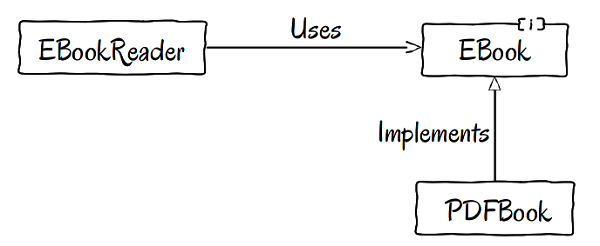
\includegraphics[scale=.4]{img/ebookreader-ebookinterface-pdfbook.png}
    \end{figure}
    \begin{exampleblock}{Good}
        \begin{itemize}
            \item Jetzt hängt \texttt{EBookReader} nur noch von einem abstrakten Interface (\texttt{EBook}) ab
            \item \texttt{PDFBook} kann nun dieses Interface implementieren und ein \texttt{EBookReader} kann somit auch ein \texttt{PDFBook} lesen
        \end{itemize}
    \end{exampleblock}

    \vspace{.1in}
    \footnotesize
    \url{http://code.tutsplus.com/series/the-solid-principles}
    \vspace{.1in}
\end{frame}

\begin{frame}{\quad}
    \center
    \Huge{\textbf{Protip \#5}}
\end{frame}

\begin{frame}{Protip \#5}
    \begin{block}{}
        \center
        \textsc{Draw diagrams.}
    \end{block}
\end{frame}

\begin{frame}{Protip \#5 Draw diagrams.}
    \begin{itemize}
        \item Diagramme können hilfreich sein, ein Problem besser zu erfassen
        \begin{itemize}
            \item Beispiele
            \item Flussdiagramme
            \item Zusammehänge zwischen verschiedenen Objekten
            \item Skizze bei geometrischen Problemen
            \item Abhängigkeiten zwischen Klassen
            \item Graphen
            \item \dots
        \end{itemize}
        \item \textit{Das Diagramm muss keinen Preis gewinnen}
    \end{itemize}
\end{frame}

\begin{frame}{\quad}
    \center
    \Huge{\textbf{Protip \#6}}
\end{frame}

\begin{frame}{Protip \#6}
    \begin{block}{}
        \center
        \textsc{Do not query.}
    \end{block}
\end{frame}

\begin{frame}{Protip \#6 Do not query.}
    \begin{itemize}
        \item Objekte sollten sich ihrem Zustand entsprechend \textbf{verhalten}
        \begin{itemize}
            \item \textit{Starte Mikrowelle mit offener Tür $\Rightarrow$ Mikrowelle erkennt Zustand und startet nicht}
        \end{itemize}
        \vspace{.2in}
        \item Objekte sollten \textit{nicht} ihrem Zustand entsprechend verwendet werden
        \begin{itemize}
            \item \textit{Überprüfe Tür der Mikrowelle $\Rightarrow$ Starte Mikrowelle, falls nicht offen}
        \end{itemize}
    \end{itemize}
\end{frame}

\begin{frame}[fragile]{Protip \#6 Do not query.}
    \begin{alertblock}{Bad}
        \begin{lstlisting}[language=Java,basicstyle=\scriptsize]
class Article {
    private int stock;

    public int getStock() {
        return this.stock;
    }

    public void sell(int quantity) {
        this.stock -= quantity;
    }
}

if (article.getStock() >= quantity) {
    article.sell(quantity);
} else {
    System.out.println("This article is currently unavailable.");
}
        \end{lstlisting}
    \end{alertblock}
\end{frame}

\begin{frame}[fragile]{Protip \#6 Do not query.}
    \begin{alertblock}{Still bad}
        \begin{lstlisting}[language=Java,basicstyle=\scriptsize]
class Article {
    private int stock;

    public void sell(int quantity) {
        if (this.stock >= quantity) {
            this.stock -= quantity;
        } else {
            System.out.println("This article is currently unavailable.");
        }
    }
}

article.sell(quantity);
        \end{lstlisting}
    \end{alertblock}
\end{frame}

\begin{frame}[fragile]{Protip \#6 Do not query.}
    \begin{exampleblock}{Good}
        \begin{lstlisting}[language=Java,basicstyle=\scriptsize]
class Article {
    private int stock;

    public boolean sell(int quantity) {
        if (this.stock >= quantity) {
            this.stock -= quantity;
            return true;
        }
        return false;
    }
}

if (!article.sell(quantity)) {
    System.out.println("This article is currently unavailable.");
}
        \end{lstlisting}
    \end{exampleblock}
\end{frame}

\begin{frame}[fragile]{Protip \#6 Do not query.}
    \begin{block}{Even better}
        \begin{lstlisting}[language=Java,basicstyle=\scriptsize]
class Article {
    private int stock;

    public boolean sell(int quantity) {
        if (quantity <= 0) {
            throw new IllegalArgumentException(
                "Negative or null quantity was given.");
        }
        if (quantity > this.stock) {
            return false;
        }
        this.stock -= quantity;
        return true;
    }
}

if (!article.sell(quantity)) {
    System.out.println("This article is currently unavailable.");
}
        \end{lstlisting}
    \end{block}
\end{frame}

\begin{frame}{\quad}
    \center
    \Huge{\textbf{Protip \#7}}
\end{frame}

\begin{frame}{Protip \#7}
    \begin{block}{}
        \center
        \textsc{Avoid floating point numbers if possible.}
    \end{block}
\end{frame}

\begin{frame}{Protip \#7 Avoid floats.}
    \begin{itemize}
        \item Man sollte sich immer überlegen, ob man Gleitkommazahlen verwenden möchte
        \item Gleitkommazahlen können tü­ckisch sein. (i.e., Genauigkeit, Epsilon-Vergleich)
        \item Gleitkommazahlen sind rechenaufwendiger als ganze Zahlen
        \item Ein paar Beispiele:
        \begin{itemize}
            \item Man kann \euro 1.99 auch einfach als Ganzzahl (199) darstellen
            \item Das Vergleichen von Abständen zwischen Punkten geht auch ohne die euklidische Norm
            $\sqrt{(x_0 - x_1)^2 + (y_0 - y_1)^2}$ mit samt der Wurzel als Gleitkommazahl zu berechnen\\
            Es genügt, wenn man $(x_0 - x_1)^2 + (y_0 - y_1)^2$ berechnet\\
            Bei ganzzahligen Koordinaten ist das Ergebnis wieder eine ganze Zahl
        \end{itemize}
    \end{itemize}
\end{frame}

\begin{frame}{\quad}
    \center
    \Huge{\textbf{Protip \#8}}
\end{frame}

\begin{frame}{Protip \#8}
    \begin{block}{}
        \center
        \textsc{Datenkapselung}
    \end{block}
\end{frame}

\begin{frame}{Protip \#8 Datenkapselung}
    \begin{itemize}
        \item Attribute sollten \textbf{immer} \texttt{private} (manchmal \texttt{protected}) sein
        \item Getter und Setter (nur wenn sinnvoll) verwenden
        \item Im Konstruktor bzw. Setter kann überprüft werden, ob übergebene Werte sinnvoll sind
        \item Nur die Methoden auf \texttt{public} setzen, welche auch von außen sichtbar sein müssen
        \item So wenig wie möglich (am besten garnichts) über Implementierungsdetails preisgeben
        \item Beim Entwurf einer Klasse, auch die Perspektive des Clients berücksichtigen und sich die Fragen stellen:\\
        \begin{itemize}
            \item Was muss ich wissen, um diese Klasse sinnvoll zu verwenden?
            \item Welche Methoden/Schnittstelle benötige ich?
            \item Gibt es evtl. unnötige Details, die nach außen sichtbar sind?
        \end{itemize}

    \end{itemize}
\end{frame}

\begin{frame}{\quad}
    \center
    \Huge{\textbf{Protip \#9}}
\end{frame}

\begin{frame}{Protip \#9}
    \begin{block}{}
        \center
        \textsc{Unterscheide zwischen\\ \textbf{Datenstrukturen} und \textbf{abstrakten Datentypen}.}
    \end{block}
\end{frame}

\begin{frame}{Protip \#9 Datenstruktur vs. abstrakter Datentyp}
    \begin{itemize}
        \item Eine \textbf{Datenstruktur} ist eine konkrete Anordnung/Organisation/Speicherung von Daten im Rechner
        \vspace{.2in}
        \item \textbf{Abstrakte Datentypen} hingegen verraten nichts über eine mögliche Implementierung
    \end{itemize}
\end{frame}

\begin{frame}{Protip \#9 Datenstruktur vs. abstrakter Datentyp}
    Quiz: \textbf{Datenstruktur} oder \textbf{abstrakter Datentyp}?
    \begin{itemize}
        \item Queue
        \item Stack
        \item Heap
        \item Map
        \item PriorityQueue
        \item HashMap
        \item Array
        \item Graph
    \end{itemize}
\end{frame}

\begin{frame}{Protip \#9 Datenstruktur vs. abstrakter Datentyp}
    \quad
    \begin{itemize}
        \item Queue $\rightarrow$ \alert{abstrakter Datentyp}
        \item Stack $\rightarrow$ \alert{abstrakter Datentyp}
        \item Heap $\rightarrow$ \alert{Datenstruktur}
        \item Map $\rightarrow$ \alert{abstrakter Datentyp}
        \item Priority Queue $\rightarrow$ \alert{abstrakter Datentyp}
        \item Hash Map $\rightarrow$ \alert{Datenstruktur}
        \item Array $\rightarrow$ \alert{Datenstruktur}
        \item Graph $\rightarrow$ \alert{abstrakter Datentyp}
    \end{itemize}
\end{frame}

\begin{frame}{\quad}
    \center
    \Huge{\textbf{Protip \#10}}
\end{frame}

\begin{frame}{Protip \#10}
    \begin{block}{}
        \center
        \textsc{Verwende aussagekräftige Bezeichner.}
    \end{block}
\end{frame}

\begin{frame}{\quad}
    \center
    \Huge{\textbf{Protip \#11}}
\end{frame}

\begin{frame}{Protip \#11}
    \begin{block}{}
        \center
        \textsc{Exceptions sind Ausnahmesituationen, nicht Kontrollfluss.}
    \end{block}
\end{frame}

\begin{frame}{\quad}
    \center
    \Huge{\textbf{Protip \#12}}
\end{frame}

\begin{frame}{Protip \#12}
    \begin{block}{}
        \center
        \textsc{Comment your code.}
    \end{block}
\end{frame}

\begin{frame}{Protip \#12 Comment your code.}
    \begin{figure}
        
\includegraphics[scale=.6]{img/zerocomments.png}
        \caption{\footnotesize{theprofoundprogrammer.com}}
    \end{figure}
\end{frame}


\begin{frame}{Protip \#12 Comment your code.}
    \begin{itemize}
        \item Kommentare beschreiben \textbf{Logik}, nicht Java-Syntax
        \item Javadoc verwenden!
        \begin{itemize}
            \item Kurz die Aufgabe der Klasse/Methode beschreiben
            \item Parameter (Typ und Semantik) (\texttt{@param})
            \item Rückgabewert (Typ und Semantik) (\texttt{@return})
            \item Exceptions? (\texttt{@throws})
        \end{itemize}
    \end{itemize}
\end{frame}

\begin{frame}[fragile]{Protip \#12 Comment your code.}
    \begin{itemize}
        \item Kommentare beschreiben Logik, nicht Java-Syntax
    \end{itemize}
    \begin{columns}[c]
        \column{.5\textwidth}
        \begin{alertblock}{Not so good}
            \begin{lstlisting}[language=Java,basicstyle=\scriptsize]
// check if a bigger than b
if (a > b) {
    // check if a bigger than c
    if (a > c) {
        // returns a
        return a;
    }
    // returns c
    return c;
// check if b bigger than c
} else if (b > c) {
    // returns b
    return b;
}
// returns c
return c;
            \end{lstlisting}
        \end{alertblock}
        \column{.5\textwidth}
        \begin{exampleblock}{Better}
            \begin{lstlisting}[language=Java,basicstyle=\scriptsize]
// return the maximum of a, b, and c
if (a > b) {
    if (a > c) {
        return a;
    }
    return c;
} else if (b > c) {
    return b;
}
return c;
            \end{lstlisting}
        \end{exampleblock}
    \end{columns}
\end{frame}

\begin{frame}[fragile]{Protip \#12 Comment your code.}
    \begin{itemize}
        \item Javadoc verwenden!
    \end{itemize}
    \begin{exampleblock}{Klasse}
        \begin{lstlisting}[language=Java,basicstyle=\tiny]
/**
 * Recursive descent parser for the recommend command.
 *
 * @version 1.1
 * @author YouniS Bensalah <younis.bensalah@riseup.net>
 */
class RecommendParser { ... }
        \end{lstlisting}
    \end{exampleblock}
\end{frame}

\begin{frame}[fragile]{Protip \#12 Comment your code.}
    \begin{itemize}
        \item Javadoc verwenden!
    \end{itemize}
    \begin{exampleblock}{Methode}
        \begin{lstlisting}[language=Java,basicstyle=\tiny]
/**
 * Parse the term and return its meaning, i.e., a set of Products.
 *
 * @param code The line containing the term.
 * @return The set of recommended Products.
 * @throws SyntaxException if the term did not match the specified syntax rules.
 * @throws InvalidNodeException if the required node does not exist.
 */
public Set<Product> parse(String code) throws SyntaxException, InvalidNodeException { ... }
        \end{lstlisting}
    \end{exampleblock}
\end{frame}

\begin{frame}{\quad}
    \center
    \Huge{\textbf{Protip \#13}}
\end{frame}

\begin{frame}{Protip \#13}
    \begin{block}{}
        \center
        \textsc{Avoid Tour-de-France code.}
    \end{block}
\end{frame}

\begin{frame}{Protip \#13 Avoid Tour-de-France code.}
    \begin{columns}[c]
        \column{.5\textwidth}
        \begin{block}{}
            \center
            \textsc{Avoid Tour-de-France code.}
        \end{block}
        \begin{itemize}
            \item Langen, unübersichtlichen Code in sinnvolle Methoden aufteilen
            \item Max. 30 Zeilen in einer Methode
            \item Tiefe Verschachtelung vermeiden!
        \end{itemize}
        \column{.5\textwidth}
        \begin{figure}
            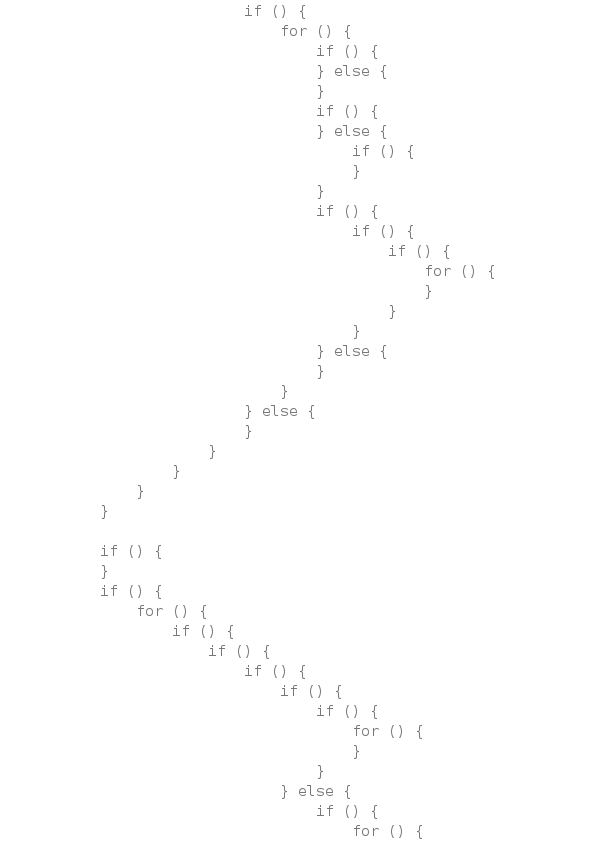
\includegraphics[scale=.3]{img/tourdefrancecode1.png}
        \end{figure}
    \end{columns}
\end{frame}

\begin{frame}{Protip \#13 Avoid Tour-de-France code.}
    \begin{itemize}
        \item \textit{Tour-de-France code}
    \end{itemize}

    \begin{figure}
        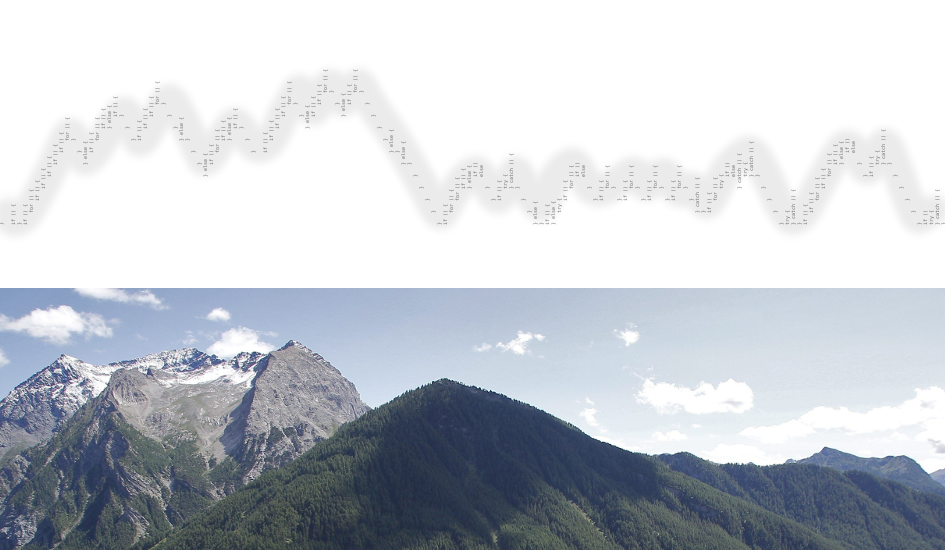
\includegraphics[scale=.4]{img/tourdefrancecode2.png}
    \end{figure}
\end{frame}

\begin{frame}{\quad}
    \center
    \Huge{\textbf{Protip \#14}}
\end{frame}

\begin{frame}{Protip \#14}
    \begin{block}{}
        \center
        \textsc{Use enums.}
    \end{block}
\end{frame}

\begin{frame}{Protip \#14 Use enums.}
    \begin{itemize}
        \item \texttt{if (today == Day.FRIDAY)} ist lesbarer als \texttt{if (today == 5)}
        \item Es schleichen sich nicht so leicht Fehler ein
        \begin{itemize}
            \item Ist \quotes{Montag} oder \quotes{Sonntag} der erste Tag der Woche?
            \item Fängt man hier bei 0 oder bei 1 an zu zählen?
            \item Welche Werte sind nochmal gültig?
        \end{itemize}
    \end{itemize}
\end{frame}

\begin{frame}{\quad}
    \center
    \Huge{\textbf{Protip \#15}}
\end{frame}

\begin{frame}{Protip \#15}
    \begin{block}{}
        \center
        \textsc{Checkstyle}
    \end{block}
\end{frame}

\begin{frame}{\quad}
    \center
    \Huge{\textbf{Protip \#16}}
\end{frame}

\begin{frame}{Protip \#16}
    \begin{block}{}
        \center
        \textsc{Test your code.}
    \end{block}
\end{frame}

\begin{frame}{Protip \#16}
    \begin{alertblock}{}
        \center
        \Huge{\textsc{Always test your code.}}
    \end{alertblock}
\end{frame}

\begin{frame}{Protip \#16 Test your code.}
    \textsc{\LARGE{Murphy's law}}\\
    \textsc{Anything that can go wrong will go wrong.}
\end{frame}

\begin{frame}{Protip \#16 Test your code.}
    \textsc{\LARGE{Corollary}}\\
    \textsc{If there is a possibility of several things going wrong, the one that will cause the most damage will be the one to go wrong.}
\end{frame}

\begin{frame}{Protip \#16 Test your code.}
    \textit{Was habe ich davon?}
    \begin{itemize}
        \item Software-Fehler finden um diese dann zu korrigieren
        \item Möglichst viele verschiedene Situationen abdecken, in denen etwas schieflaufen kann
    \end{itemize}
\end{frame}

\begin{frame}{Protip \#16 Test your code.}
    \textit{Wann habe ich mein Programm genug getestet?}
    \pause
    \begin{itemize}
        \item Nie.
        \pause
        \item Die sinnvollere Frage lautet: \quotes{\textbf{Wie sehen gute Testfälle aus?}}
    \end{itemize}
\end{frame}

\begin{frame}{Protip \#16 Test your code.}
    \textit{Ok, dann halt: wie sehen gute Testfälle aus?}
    \pause
    \begin{itemize}
        \item Prüfen genau eine spezifische Eigenschaft ab
        \item Kurz und knapp
        \item Können isoliert ausgeführt werden
        \item Orientieren sich an der Spezifikation (i.e., Aufgabenstellung \textit{nicht} Implementierung)
        \item Typische Vorgehensweise:
        \begin{enumerate}
            \item Klassifizierung der möglichen Eingabedaten
            \begin{itemize}
                \item Standardsituationen und Randfälle betrachten
            \end{itemize}
            \item Auswahl der repräsentativen Daten zu jedem Testfall
        \end{enumerate}
    \end{itemize}
\end{frame}


\begin{frame}{Protip \#16 Test your code.}
    \Large{\quotes{Testing shows the presence, not the absence of bugs.}}\\
    \vspace{.4in}
    \textit{- Dijkstra}
\end{frame}

\begin{frame}{Protip \#16}
    \begin{alertblock}{}
        \center
        \Huge{\textsc{Did I say you should always test your code?}}
    \end{alertblock}
\end{frame}

\begin{frame}{\quad}
    \center
    \Huge{\textbf{Protip \#17}}
\end{frame}

\begin{frame}{Protip \#17}
    \begin{block}{}
        \center
        \textsc{Use Breakpoints.}
    \end{block}
\end{frame}

\begin{frame}{Protip \#17 Use Breakpoints.}
    \begin{itemize}
        \item \textbf{Breakpoints} (Haltepunkte) erleichtern das finden von Fehlerursachen im Quellcode
        \item Idee: Programm \quotes{in Zeitlupe} laufen lassen
        \item Vorgehensweise:
        \begin{enumerate}
            \item Setze \textbf{Breakpoint} an \quotes{kritische} Stelle im Code
            \item Führe das Programm im \textbf{Debug-Modus} aus
            \item Das Programm wird an der markierten Stelle \alert{pausieren}
            \item Der Programmierer hat die Chance, den Zustand es Programms zu untersuchen und nach Anomalien zu suchen
            \begin{itemize}
                \item Inhalt von Variablen anschauen
                \item Weiterlaufen bis zum nächsten Breakpoint
            \end{itemize}
        \end{enumerate}
        \item Alle gängigen IDEs (Eclipse, NetBeans, \dots) unterstützen das Setzen von Breakpoints
    \end{itemize}
\end{frame}

\begin{frame}{Protip \#17 Use Breakpoints.}
    \begin{figure}
        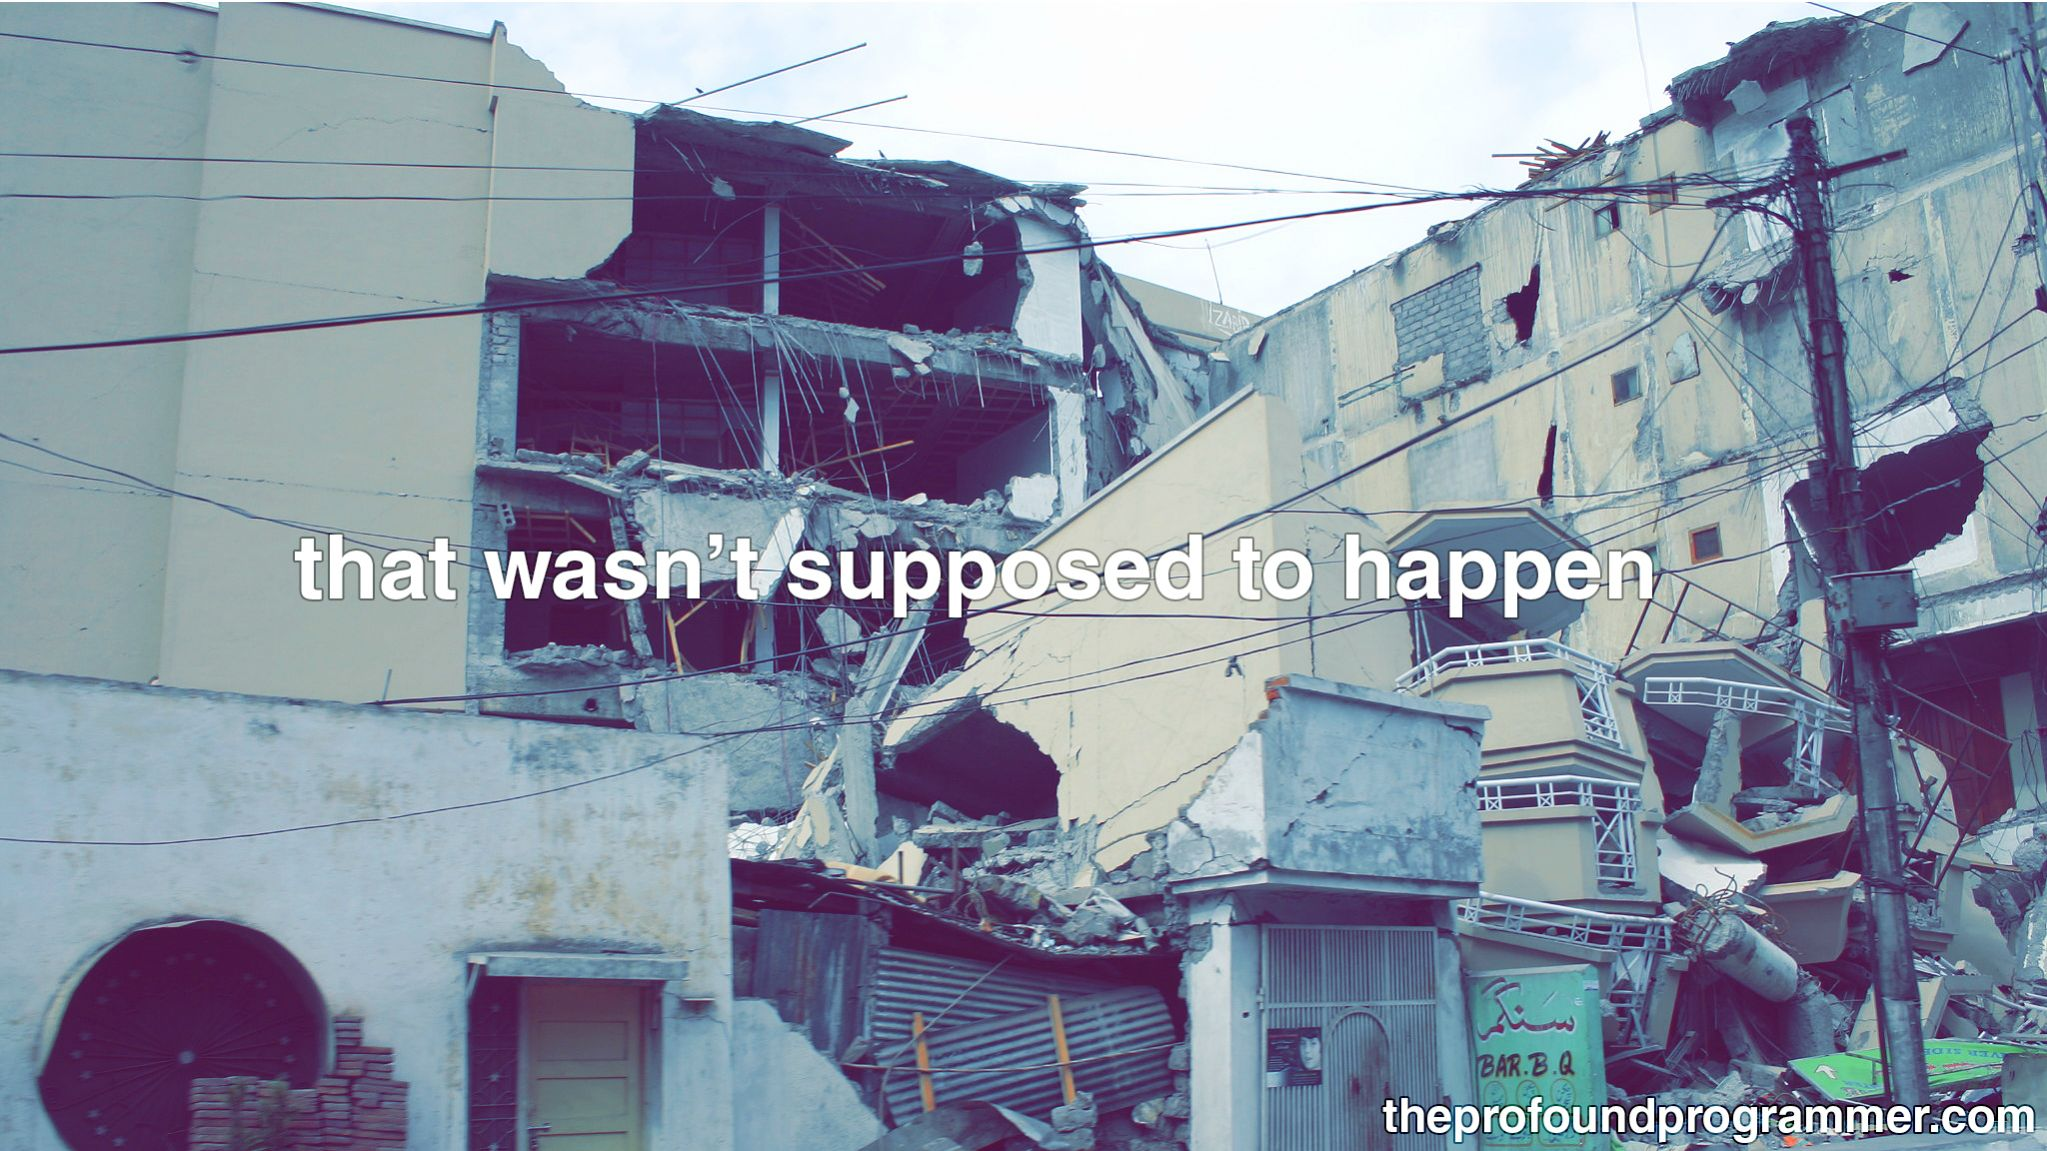
\includegraphics[scale=.15]{img/NG8XW8J8GT.jpg}
        \caption{\footnotesize{theprofoundprogrammer.com}}
    \end{figure}
\end{frame}

\section{and stuff}

\begin{frame}{\quad}
    \center
    \Huge{Typische Probleme und (hoffentlich) sinnvolle Lösungen}
\end{frame}

\begin{frame}{\quad}
    \center
    Was auch immer das heißen soll\dots
\end{frame}

\begin{frame}[fragile]{Duplikate in Array/List}
    \begin{itemize}
        \item \textbf{Problem:} Bestimme, ob ein \texttt{Array} bzw. eine \texttt{List} doppelte Elemente enthält
        \vspace{.2in}
    \begin{lstlisting}[language=Java,basicstyle=\scriptsize]
String[] fruitArray = {
    "Apfel",
    "Mango",
    "Ananas",
    "Orange",
    "Apfel",
    "Kiwi",
    "Birne",
    "Apfel",
    "Orange"
};
    \end{lstlisting}

    \end{itemize}

\end{frame}

\begin{frame}[fragile]{Duplikate in Array/List}
    \begin{itemize}
        \item \textbf{Lösung:} Füge alle Elemente in ein \texttt{Set} ein und vergleiche dann die Größe von \texttt{Set} und \texttt{Array}

        \vspace{.2in}

        \begin{lstlisting}[language=Java,basicstyle=\scriptsize]
String[] fruitArray = { ... };

Set<String> fruitSet = new HashSet<>(Arrays.asList(fruitArray));

if (fruitSet.size() == fruitArray.length) {
    System.out.println("No duplicates.");
} else {
    System.out.println("Duplicates.");
}
        \end{lstlisting}

\begin{exampleblock}{}
\begin{lstlisting}[language=Java,basicstyle=\scriptsize]
Duplicates.
\end{lstlisting}

\end{exampleblock}


    \end{itemize}
\end{frame}


\begin{frame}[fragile]{Klammern parsen}
    \begin{itemize}
        \item \textbf{Problem:} Bestimme, ob ein Klammerausdruck gültig ist
    \end{itemize}
\end{frame}

\begin{frame}[fragile]{Klammern parsen}
    \begin{itemize}
        \item \textbf{Lösung:} Verwende einen \texttt{Stack}!
    \end{itemize}

    \begin{lstlisting}[language=Java,basicstyle=\scriptsize]
boolean parseParens(String input) {
    Stack<Character> parens = new Stack<>();
    for (int i = 0; i < input.length(); i++) {
        char c = input.charAt(i);
        if (c == '(') {
            parens.push('(');
        } else if (c == ')') {
            if (parens.empty() || parens.peek() != '(') {
                return false;
            }
            parens.pop();
        } else {
            return false;
        }
    }
    return parens.empty();
}

parseParens("(())()((()()))()");  // true
parseParens("(()()))()(");  // false
    \end{lstlisting}
\end{frame}

\begin{frame}{Eigene Exception mit Message}
    \begin{itemize}
        \item \textbf{Problem:} Eigene Exception schreiben, aber (wie bei \texttt{java.lang.Exception}) eine Nachricht an Konstruktor übergeben
    \end{itemize}
\end{frame}

\begin{frame}[fragile]{Eigene Exception mit Message}
    \begin{itemize}
        \item \textbf{Lösung:} Verwende den Konstruktor der Oberklasse
    \end{itemize}

\begin{block}{}
    \begin{lstlisting}[language=Java,basicstyle=\scriptsize]
public class IllegalGameStateException extends Exception {

    public IllegalGameStateException(String message) {
        super(message);
    }

}
    \end{lstlisting}
\end{block}


\end{frame}

\begin{frame}[fragile]{Eigene Exception mit Message}
    \begin{exampleblock}{Beispiel}
        \begin{lstlisting}[language=Java,basicstyle=\scriptsize]
Cell target = this.fetch(x, y);

if (target == Cell.OFF) {
    throw new IllegalGameStateException(String.format(
            "Cannot place an ant at position (%s, %s). " +
            "Coordinates are off the grid.", x, y));
}
        \end{lstlisting}
    \end{exampleblock}

\end{frame}

\appendix
\beginbackup

\begin{frame}{Fragen?}
    \begin{figure}
        
\includegraphics[scale=.4]{img/iknowjava.jpg}
    \end{figure}
\end{frame}

\begin{frame}{\quad}
    \center
    \Large{Es hat mir Spaß gemacht}
\end{frame}

\begin{frame}{Bis irgendwann\dots}
    \begin{figure}
        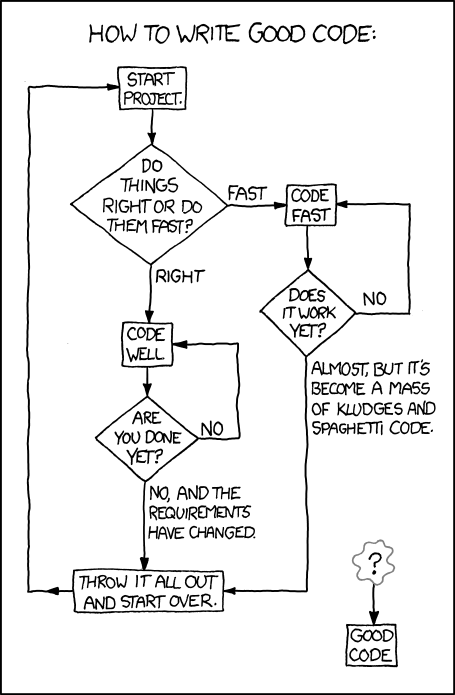
\includegraphics[scale=.3]{img/good_code.png}
        \caption{\footnotesize{xkcd.com}}
    \end{figure}
\end{frame}

\backupend

\end{document}
